\begin{appendices}
\appendixpage
\noappendicestocpagenum
\addappheadtotoc

\pretocmd{\chapter}{%
  \clearpage
  \pagenumbering{arabic}%
  \renewcommand*{\thepage}{\thechapter\arabic{page}}%
}{}{}

\chapter{Body orientation conventions}\setlength{\parindent}{0pt}
\section{Introduction}

\begin{figure}[ht]
    \centering
    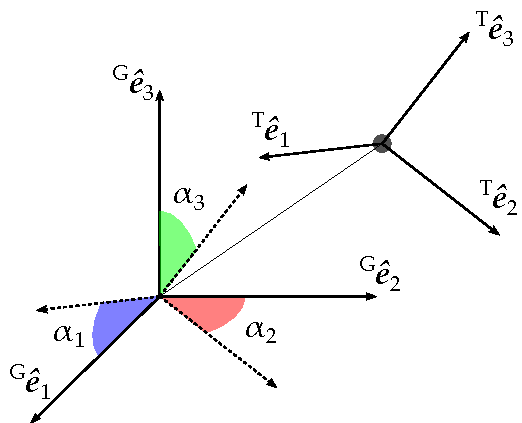
\includegraphics{img/XX_appendices/xx_01.pdf}
    \caption{Depiction of a fixed (global -- superscript $G$) and a moving (technical -- superscript $T$) coordinate system and their relative orientation, expressed as generic angles $\alpha_1$, $\alpha_2$, and $\alpha_3$. The technical coordinate system is supposed to be rigidly attached to the body (gray dot) it refers to.}
    \label{fig:coordinate_systems_general}
\end{figure}

Body orientation in three-dimensional space can be expressed with different approaches, all having in common the concept of \textit{coordinate systems} (CSs). A coordinate system is commonly defined as a right-handed, orthonormal base $\mathcal{C} = \begin{Bmatrix} \hb{e}_1 & \hb{e}_2 & \hb{e}_3 \end{Bmatrix}$. 

For objects moving in small-sized environment (e.g. a laboratory), a suitable solution to compute orientation is to express it using two distinct CSs, one embedded into the object, the other fixed, hence to compute their relative orientation (Figure \ref{fig:coordinate_systems_general}). For the sake of simplicity, the fixed and embedded CSs will be named the global and the technical CS, denoted as ${^G}{}\mathcal{C}$ and ${^T}{}\mathcal{C}$.

Nonetheless, many representation are made possible through different mathematical objects. In the following sections, the main ones are presented, along with the relationships allowing to shift from one representation to another. 

%% ------------------------------------ %%
\section{Direction cosine matrices}
\begin{proposition}
It is possible to know the orientation of a rigid body relative to a global coordinate system ${^G}{}\mathcal{C} = \begin{Bmatrix} {^G}{}\hb{e}_1 & {^G}{}\hb{e}_2 & {^G}{}\hb{e}_3 \end{Bmatrix} \iff \exists\ $ an orthonormal base ${^T}{}\mathcal{C} = \begin{Bmatrix} {^T}{}\hb{e}_1 & {^T}{}\hb{e}_2 & {^T}{}\hb{e}_3 \end{Bmatrix}$ rigidly fixed with it.
\end{proposition}

Given the latter proposition, it is possible to establish a linear relationship between the two CSs for each of their components. Such relationship can be expressed in the following form:

\begin{equation}\label{eq:dcm_01}
    R_{ij} = {^G}{}\hb{e}_i \cdot {^T}{}\hb{e}_j \quad \quad i,j = 1, \dots, 3
\end{equation}

Being the CSs components unit vectors by definition, equation (\ref{eq:dcm_01}) is equivalent to find the cosine of the angle that ${^T}{}\hb{e}_j$ forms with ${^G}{}\hb{e}_i$. Indeed, the terms $R_{ij}$ are referred to as the \textit{direction cosines}.

It is possible to combine all the nine $R_{ij}$ into a linear transformation matrix, named \textit{direction cosine matrix} (DCM) or \textit{rotation matrix}:

\begin{equation}\label{eq:dcm_02}
    \bm{R} = \begin{bmatrix}R_{11} & R_{12} & R_{13}\\
    R_{21} & R_{22} & R_{23}\\
    R_{31} & R_{32} & R_{33}\end{bmatrix}
\end{equation}

The DCM given by (\ref{eq:dcm_02}) allows to transform each ${^T}{}\hb{e}_j$ into the corresponding ${^G}{}\hb{e}_i$. Indeed, from equation (\ref{eq:dcm_01}) one has:

\begin{equation}\label{eq:dcm_03}
    {^T}{}\hb{e}_i = \bm{R}\: {^G}{}\hb{e}_i
\end{equation}

To obtain the opposite rotation, one has:

\begin{equation}\label{eq:dcm_04}
    {^G}{}\hb{e}_i = \bm{R}^T\: {^T}{}\hb{e}_i 
\end{equation}

%% ------------------------------------ %%

\section{Euler angles}
The \textit{Euler angles} representation allows to establish the orientation of the technical coordinate system ${^T}{}\mathcal{C} = \begin{Bmatrix} {^T}{}\hb{e}_1 & {^T}{}\hb{e}_2 & {^T}{}\hb{e}_3 \end{Bmatrix}$ relative to the fixed coordinate system ${^G}{}\mathcal{C} = \begin{Bmatrix} {^G}{}\hb{e}_1 & {^G}{}\hb{e}_2 & {^G}{}\hb{e}_3 \end{Bmatrix}$. The idea is to express the nine direction cosines as a function of three parameters only, referred to as the \textit{Euler angles}.

\begin{figure}[ht]
    \centering
    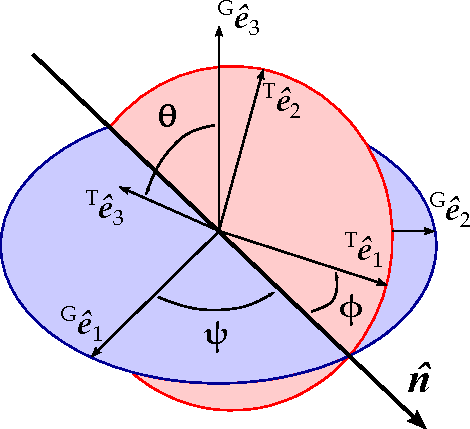
\includegraphics{img/XX_appendices/xx_02.pdf}
    \caption{Graphical representation of the \textit{line of nodes} $\hb{n}$ as the intersection of the planes perpendicular to ${^G}{}\hb{e}_3$ and ${^T}{}\hb{e}_3$. The angles $\psi$, $\theta$, and $\phi$ represent the \textit{precession}, \textit{nutation}, and \textit{intrisic rotation}, respectively.}
    \label{fig:euler_angles_general}
\end{figure}

To be applicable, the following relationship must be satisfied:

\begin{equation}
    {^G}{}\hb{e}_{3} \times {^T}{}\hb{e}_3 \neq \bm{0}
\end{equation}

That is the two unit vectors must not be parallel. In all other cases, it is always possible to define a unit vector such that:

\begin{equation}
    \hb{n} = \frac{{^G}{}\hb{e}_3 \times {^T}{}\hb{e}_3}{|| {^G}{}\hb{e}_3 \times {^T}{}\hb{e}_3 ||}
\end{equation}

Such unit vector represents the intersection between the planes perpendicular to ${^T}{}\hb{e}_3$ and ${^G}{}\hb{e}_3$, respectively, and it is referred to as the \textit{line of nodes} (Figure \ref{fig:euler_angles_general}).

From the line of nodes three angles can be defined:

\begin{itemize}
    \item \textit{Precession} $\psi$: it is the angle required to rotate  ${^T}{}\hb{e}_1$ (counterclockwise) about ${^G}{}\hb{e}_3$ to obtain $\hb{n}$;
    \item \textit{Nutation} $\theta$: it is the angle ${^T}{}\hb{e}_3$ forms with ${^G}{}\hb{e}_3$;
    \item \textit{Intrisic rotation} $\phi$: it is the angle required to rotate,  $\hb{n}$ (counterclockwise) in the plane orthogonal to ${^T}{}\hb{e}_3$ to obtain ${^T}{}\hb{e}_1$.
\end{itemize}

\subsection{Three ordered rotations}
\begin{figure}[ht]
    \centering
    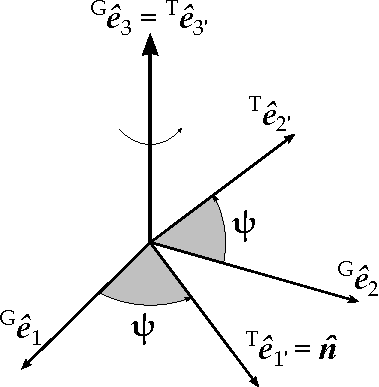
\includegraphics{img/XX_appendices/xx_03a.pdf}
    \caption{The first rotation occurring about ${^G}{}\hb{e}_3$ to obtain the precession angle $\psi$.}
    \label{fig:euler_first_rotation}
\end{figure}

\begin{figure}[ht]
    \centering
    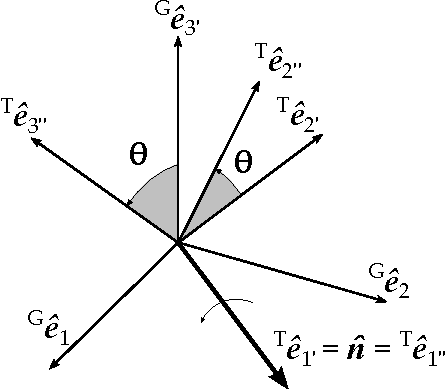
\includegraphics{img/XX_appendices/xx_03b.pdf}
    \caption{The second rotation occurring about $\hb{n} \triangleq {^T}{}\hb{e}_{1'}$ to obtain the nutation angle $\theta$.}
    \label{fig:euler_second_rotation}
\end{figure}

\begin{figure}[ht]
    \centering
    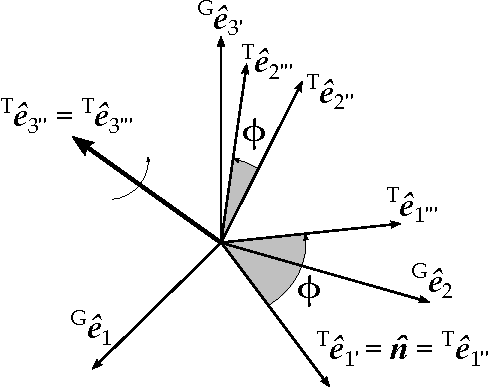
\includegraphics{img/XX_appendices/xx_03c.pdf}
    \caption{The third rotation occurring about ${^T}{}\hb{e}_{3''}$ to obtain the intrinsic rotation angle $\phi$.}
    \label{fig:euler_third_rotation}
\end{figure}

\paragraph{1$^{\rm st}$ rotation.} This rotation allows the computation of the line of nodes $\hb{n}$ by rotating ${^T}{}\mathcal{C}$ about ${^G}{}\hb{e}_1$. The angle formed ($\psi$ -- Figure \ref{fig:euler_first_rotation}) is the precession angle. A new orthonormal base has formed, ${^T}{}\mathcal{C}'$, such that:

\begin{equation}\label{eq:first_rotation}
    {^T}{}\mathcal{C}' = \begin{bmatrix} {^T}{}\hb{e}_{1'} \\ {^T}{}\hb{e}_{2'} \\ {^T}{}\hb{e}_{3'} \end{bmatrix} = 
    \begin{bmatrix}
    \cos \psi \: {^G}{}\hb{e}_1 + \sin \psi \: {^G}{}\hb{e}_2 \\
    -\sin \psi \: {^G}{}\hb{e}_1 + \cos \psi \: {^G}{}\hb{e}_2 \\
    {^T}{}\hb{e}_3
    \end{bmatrix}
\end{equation}

\paragraph{2$^{\rm nd}$ rotation.} This rotation occurs about the line of nodes $\hb{n} \triangleq {^T}{}\hb{e}_{1'}$. The angle formed by ${^T}{}\mathcal{C}'$ ($\theta$ -- Figure \ref{fig:euler_second_rotation}) is the nutation angle. A new orthonormal base has formed, ${^T}{}\mathcal{C}''$, such that:

\begin{equation}
    {^T}{}\mathcal{C}'' = \begin{bmatrix} {^T}{}\hb{e}_{1''} \\ {^T}{}\hb{e}_{2''} \\ {^T}{}\hb{e}_{3''} \end{bmatrix} = 
    \begin{bmatrix}
    {^T}{}\hb{e}_{1'}\\
    \cos \theta \: {^T}{}\hb{e}_{2'} + \sin \theta \: {^T}{}\hb{e}_{3'} \\
    -\sin \theta \: {^T}{}\hb{e}_{2'} + \cos \theta \: {^T}{}\hb{e}_{3'} \\
    \end{bmatrix}
\end{equation}

\paragraph{3$^{\rm rd}$ rotation.} The last of the three rotations occurs about ${^T}{}\hb{e}_{3''}$. The angle formed by ${^T}{}\mathcal{C}''$ ($\phi$ -- Figure \ref{fig:euler_third_rotation}) is the intrinsic rotation angle. A new base has formed, ${^T}{}\mathcal{C}'''$, such that:

\begin{equation}
    {^T}{}\mathcal{C}''' = \begin{bmatrix} {^T}{}\hb{e}_{1'''} \\ {^T}{}\hb{e}_{2'''} \\ {^T}{}\hb{e}_{3'''} \end{bmatrix} = 
    \begin{bmatrix}
    \cos \phi \: {^T}{}\hb{e}_{1''} + \sin \phi \: {^T}{}\hb{e}_{2''} \\
    -\sin \phi \: {^T}{}\hb{e}_{1''} + \cos \phi \: {^T}{}\hb{e}_{2''} \\
    {^T}{}\hb{e}_{3''}
    \end{bmatrix}
\end{equation}

\end{appendices}